\documentclass[a4paper]{article}

\usepackage[margin=1.2in]{geometry}

\usepackage[T1]{fontenc}
\usepackage[francais]{babel}
\usepackage{fontspec}
\setmainfont{Droid Serif}
\setmonofont{Inconsolata}

\usepackage{url}
\usepackage{hyperref}

\usepackage{fancyhdr}
\pagestyle{fancy}

\usepackage{graphicx}

\usepackage{minted}

\definecolor{foreground}{RGB}{21,21,21}
\definecolor{background}{RGB}{242,245,227}
\definecolor{title}{RGB}{255,31,110}
\definecolor{gray}{RGB}{155,155,155}
\definecolor{toogyblue}{RGB}{87,102,181}

\newminted{csharp}{bgcolor=gray!25,fontsize=\normalsize,mathescape,linenos,frame=lines,framerule=0.3pt}

\newcommand{\tptitle}
    {\textbf{TP BDSP 13/14} $\bullet$ T'es triste $\bullet$ \textbf{GConfs}}

\fancyhf{}
\lhead{\textbf{\thepage}}
\rhead{\tptitle{}}
\lfoot{\tptitle{}}
\rfoot{\textbf{\thepage}}
\renewcommand{\headrulewidth}{0.4pt}
\renewcommand{\footrulewidth}{0.4pt}

% END STYLE

\title{T'es triste}

\author{
    GConfs
}

\date{15 novembre 2013}

\begin{document}
\color{foreground}

%
\begin{center}
    \fbox{
        \begin{minipage}[t]{6cm}
            \begin{center}
                \textbf{\huge T'es triste} \\
                \emph{\color{gray} TP BDSP 13/14}
            \end{center}
        \end{minipage}
    }
\end{center}

\section*{Introduction}

Dans ce TP, vous allez devoir réaliser un tétris très simplifié : les pièces
sont de taille 3 (et non 4) et elles ne peuvent pas tourner. \\

\begin{center}
    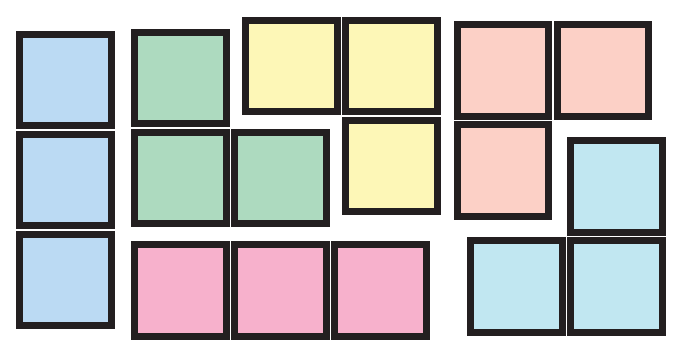
\includegraphics[scale=0.5]{img/pieces.eps}
\end{center}

Ce TP est fait pour être réalisé en équipe (2-4 membres) mais vous pouvez très
bien le faire tout seul, si vous en êtes capable (même si c'est moins marrant).
\\

\textbf{But du TP :} apprendre à utiliser \textbf{Git} à plusieurs et apprendre
les bases d'\textbf{XNA}.

\begin{center}\noindent\rule{12cm}{0.4pt}\end{center}

\tableofcontents

\begin{center}\noindent\rule{12cm}{0.4pt}\end{center}

\section{Création du dépôt Git et du projet XNA}

\noindent{\color{red} Si vous êtes bloqué à une étape, les assistants sont là pour vous
aider. Alors n'hésitez pas à leur demander.}

\begin{enumerate}
    \item Commencez par tous vous inscrire sur \url{https://bitbucket.org} ou
    \url{http://github.com} (mais tous les membres au même endroit sinon ça va
    pas le faire). \\
    Ces deux sites permettent à des développeurs d'héberger leurs dépôts Git, et ce
    gratuitement.\\
    \textbf{Attention} : GitHub ne permet pas de faire de dépôt privé
    de base; il faut un compte étudiant. Préférez BitBucket si vous n'êtes pas
    quelqu'un d'opensource.\\

    {\color{red} \textbf{Attention} : \\Les étapes \textbf{2} et \textbf{3}
    sont faites par une seule personne. Choisissez la. Les autres regardent et
    l'aident.}\\

    \item L'heureux élu se rend donc sur le site que vous avez choisi et créé un
    nouveau dépôt (en général y'a un gros bouton pour ça, vous allez y arriver). \\

    \item Cette même personne créé un nouveau projet XNA sur VS.
\end{enumerate}

\% \textbf{TODO}: Corwin doit rajouter des étapes pour l'extension Git de VS
À la fin, ils sont tous sensés avoir le nouveau projet sur leur VS. \\
Expliquer comment utiliser l'extension pour commit, push etc.

\section{Principe du jeu}

\begin{center}
    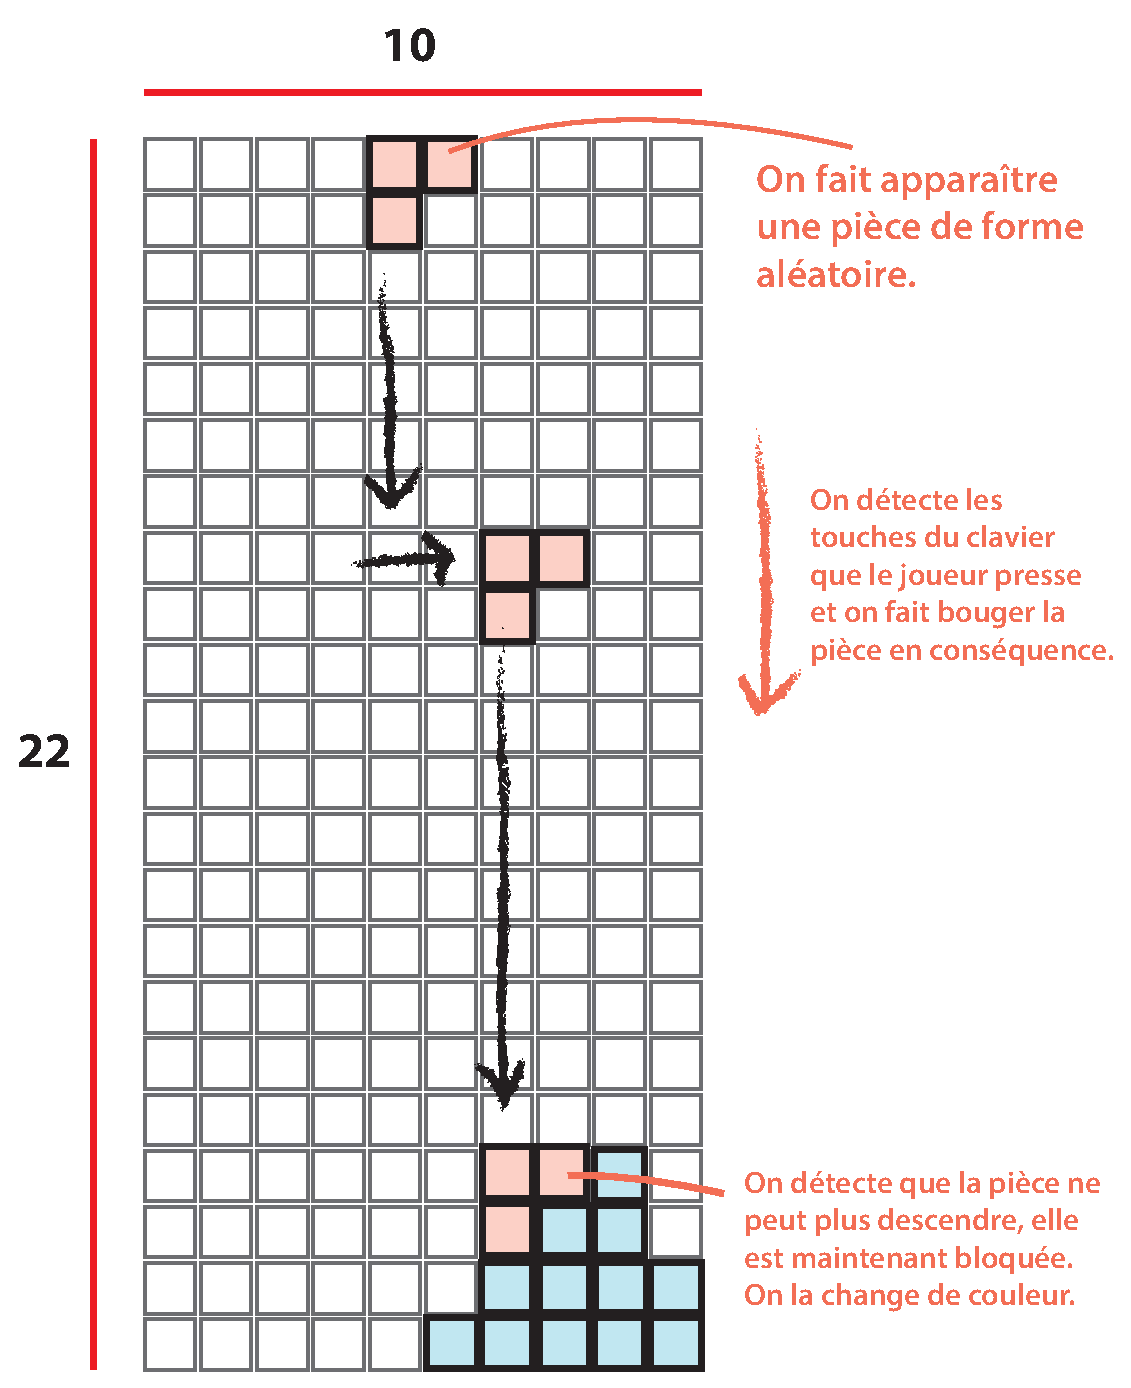
\includegraphics[scale=0.7]{img/game-explanation.eps} 
\end{center}

\noindent\textbf{Remarque} : ce processus tourne en boucle puisque quand une
pièce devient bloquée, on en fait apparaître une nouvelle qui subira le même
sort que la précédente.

\newpage
\section{Liste des fonctionnalités à implémenter}

\begin{enumerate}
    \item Plateau de jeu (map sur laquelle les pièces se déplaceront)
    \item Pièce (composée de 3 cases)
        \begin{enumerate}
            \item Génération d'une pièce aléatoire
            \item Déplacement
            \item Drop (la pièce tombe le plus bas possible et se bloque)
        \end{enumerate}
    \item Boucle de jeu principale
        \begin{enumerate}
            \item Initialisation du jeu (dans la fonction du même nom)
            \item Chargement des textures
            \item États de jeu (Running|GameOver)
            \item Détection de l'input du joueur (touches clavier)
            \item Détection du GameOver
        \end{enumerate}
\end{enumerate}

\begin{center}
    {\large\color{red} Pour vous aider, la partie \textbf{5} vous explique
    comment implémenter chaque fonctionnalité. Vous n'êtes pas obligés de vous
    en servir. Si vous voulez un peu plus de challenge vous pouvez proposer
    votre propre implémentation. :) Vous êtes libres.}
\end{center}

\section{Les images du jeu sont fournies !}

Pour les téléchargez, rendez vous ici : \url{http://too.gy/bdsp/tp.zip}.

\section{Comment implémenter tout ça}

\subsection{Plateau de jeu}

\subsubsection{Principe}

Notre plateau de jeu est composé de \textbf{10} cases sur la coordonnée x de
XNA et de \textbf{22} cases sur sa coordonnée y. (voir schéma 'Principe du jeu')\\
Pour chaque case on a envie de savoir si la case est occupée par soit :

\begin{itemize}
    \item une case vide
    \item un bloc d'une pièce bloquée (une pièce est constituée de 3 blocs)
    \item un bloc d'une pièce non-bloquée
\end{itemize}

(on différencie pièce bloquée et non-bloquée car on veut les afficher
différemment). \\

Le plus simple c'est de représenter les cases notre plateau par un tableau de
bytes : \\

\begin{csharpcode*}{label=Plate.cs}
public class Plate
{
    public byte[,] Cells { get; set; }
}
\end{csharpcode*}

Pour accéder à une case de notre plateau, il suffit alors de faire : \\

\begin{csharpcode}
Plate p = new Plate();

byte b = p.Cells[0,0]; // récupère la case tout en haut à gauche
\end{csharpcode}

Pour parcourir l'ensemble de nos cases, il suffit de faire : \\

\begin{csharpcode}
for (int x = 0; x < 10; x++)
{
    for (int y = 0; y < 22; x++)
    {
        // Valeur de la case =  p.Cells[x,y]
    }
}
\end{csharpcode}

\vspace{0.2cm}

\noindent\emph{\color{toogyblue} Si vous avez des problèmes avec toutes ces notions,
demandez aux assistants de vous les expliquer. Vous les verrez bientôt en TP,
ce sont des choses très basiques.} \\

\subsubsection{Affichage}

\begin{csharpcode*}{label=Plate.cs}
public class Plate
{
    public void Draw(SpriteBatch spriteBatch)
    {
        // On boucle sur chaque case
        // Si la case est un bloc on affiche sa texture (bloc bloqué ou en mouvement)
        // Sinon on fait rien
    }
}
\end{csharpcode*}

Il est certain que vous ferrez attention au décalage de base par rapport au
coin en haut à gauche de l'écran : \\

\begin{center}
    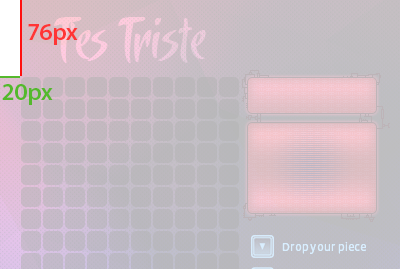
\includegraphics[scale=0.5]{img/decalage.png}
\end{center}

\subsubsection{Fonctions à implémenter}

\begin{csharpcode*}{label=Plate.cs}
public class Plate
{
    public bool IsLineFull(int y)
    {
        // Renvoie vrai si la ligne numéro y est pleine (bytes 2 ou 3)
    }
    
    public void EmptyLine(int y)
    {
        // Vide la ligne y et fait tomber tous les blocs
        // au dessus de cette ligne d'une case
    }
}
\end{csharpcode*}

\subsection{Pièce}

\subsubsection{Implémentation}

On peut considérer qu'une pièce est un ensemble de 3 blocs. Chaque bloc a des
coordonnées qui lui sont propres sur la map, soit un couple x,y. \\

Pour plus de clarté, on va déclarer une structure (si vous ne savez pas ce que
c'est, considérez que c'est comme une classe) :

\begin{csharpcode*}{label=Piece.cs}
public class Piece
{
    public Cell[] Cells { get; set; }

    public struct Cell
    {
        public byte X { get; set; }
        public byte Y { get; set; }

        public Cell(byte x, byte y)
        {
            X = x;
            Y = y;
        }
    }
}
\end{csharpcode*}

\subsubsection{Déplacement}

Pour pouvoir se déplacer, la pièce a besoin de savoir sur quel plateau de jeu
elle est. On va donc lui rajouter le plateau en attribut. On donnera une valeur
à cet attribut au moment de la création de la pièce, dans le constructeur donc.

\begin{csharpcode*}{label=Piece.cs}
public class Piece
{
    private Plate _plate;

    public Piece(Plate plate)
    {
        _plate = plate;
    }
}
\end{csharpcode*}

\section{Bonus}

Si vous êtes vraiment des malades et que vous avez tout fait, vous pouvez vous
amuser à implémenter ces quelques fonctionnalités supplémentaires :

\begin{enumerate}
    \item Rajout d'un état de jeu 'Pause'
    \item Scoring
        \begin{enumerate}
            \item Calcul du score
            \item Affichage du score (SpriteFont XNA)
        \end{enumerate}
    \item Piece holding (le joueur garde une pièce en mémoire)
\end{enumerate}

%

\end{document}

